% Penser une application pour la détection d'objet

\subsection{Une interface pour le traitement des sources}
    \subsubsection{Construire une application réutilisable}
    La création d'un modèle performant est une base essentielle à tout projet intégrant l'\ia à sa chaîne de traitement des sources : il s'agit du socle sur lequel repose l'efficacité des outils développés pour les chercheurs. Cependant, d'un point de vue pratique, les historiens n'interagissent pas directement avec ce modèle, il est donc nécessaire de développer une application qui sert de pont entre les utilisateurs et l'algorithme de détection, et qui permet ainsi le dépôt et le traitement des sources par l'intermédiaire d'une interface graphique, accessible et utilisable par les chercheurs\footnote{Les applications \eida et \vhs sont développées en prenant en considération leur utilisation future par un public plus large que les chercheurs affiliés à ces projets. Elles restent cependant axées, dans leur développement, à un public provenant du monde de la recherche, nous utilisons donc le terme \og chercheur \fg pour décrire ses utilisateurs. D'autres projets, tels que le projet \href{https://filigranes.hypotheses.org/}{Filigranes pour tous}, développent leurs outils autour des utilisateurs grand public ; nous les prenons en compte dans ce mémoire, en ayant conscience de la différence de réflexion que cela apporte sur la manière de construire une plateforme.}. Cette plateforme doit ainsi être développée en prenant en compte la diversité des sources étudiées par ses utilisateurs.
    
    La détection d'objet dans les images représente une première étape de nombreuses tâches de vision artificielle, et présente ainsi un intérêt pour de nombreux projets aux objectifs divers. Le développement d'une application pour la détection d'objet dans des images est donc d'intérêt pour plusieurs projets en cours, tels que \vhs et \eida : pour éviter à de multiples projets de développer des outils aux fonctionnalités similaires, ces deux projets ont fait le choix de construire une application réutilisable, dont le code sera proposé en accès libre sur GitHub\footnote{Le développement des applications \eida et \vhs étant toujours en cours, le code n'est à cette date par disponible en accès libre.}. Le développement des applications \eida et \vhs est collaboratif, porté par les ingénieurs des deux projets qui travaillent en parallèle pour la mise en place d'une plateforme adaptée aux besoins de chacun des projets : l'enjeu est donc de créer une application suffisamment spécifique pour répondre aux besoins des deux projets, tout en étant suffisamment généraliste pour être réemployée à l'avenir par d'autres projets.
    
    Il n'a, à ce jour, pas été développé d'interface pour les applications \eida et \vhs. Ces dernières sont accessibles pour les chercheurs qui demandent aux équipes d'ingénierie la création d'un identifiant donnant accès à l'interface administrateur des applications : celles-ci reposent sur l'interface par défaut proposée par Django (fig. \ref{fig:eida_admin}). Un développement spécifique des interfaces destinées aux utilisateurs\footnote{Le développement web frontal, ou \textit{front-end}, désigne les productions d'une application avec lesquelles l'utilisateur peut interagir directement.} est prévu, afin de rendre ces applications plus ergonomiques. L'objectif actuel étant de mettre à disposition des chercheurs partenaires des applications pour le dépôt et le traitement de leurs sources, celles-ci ne sont pas accessibles au grand public, et ont pour objectif de permettre la constitution de jeux de données d'entraînement par le biais d'une interface graphique. 
    
    \begin{figure}[h]
    	\centering
    	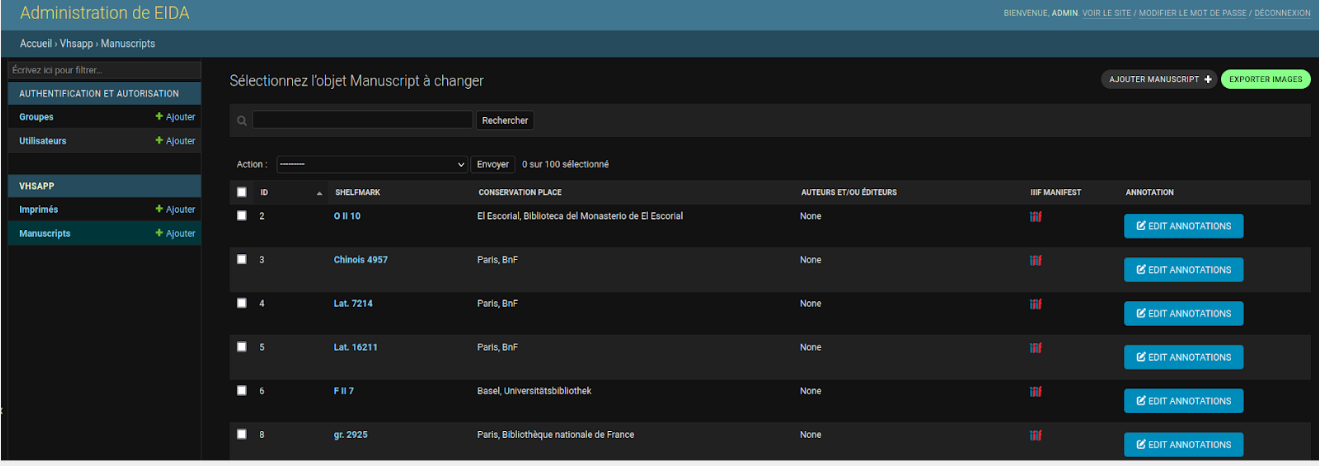
\includegraphics[width=16cm]{images/eida_admin.png}
    	\caption{Interface administrateur de l'application \eida}
    	\label{fig:eida_admin}
    \end{figure}
    
    \subsubsection{Développement en collaboration, programmation modulaire et remploi du code}
    Dans ce contexte, les ingénieurs des projets \eida et \vhs travaillent sur différentes branches d'un même dépôt GitHub, qui dispose alors d'une branche pour la mise en production de l'application \eida et d'une autre pour la mise en production de l'application \vhs. Ainsi, il est possible pour un projet d'exploiter les développements faits dans le cadre du second, ou de choisir de ne pas les employer s'ils ne semblent pas pertinents pour les besoins spécifiques du projet concerné. Ce développement collaboratif par le biais d'un dépôt GitHub assure une liaison constante entre les équipes des deux projets, tout en offrant la liberté de ne pas mettre en production tous les développements faits dans le cadre du projet jumeau.
    
    La programmation modulaire est une solution favorisée pour la création d'une application réutilisable, puisqu'elle permet le développement de modules indépendants qui répondent à des besoins spécifiques, et qui peuvent être réemployés par d'autres projets sans être dépendants du reste de l'application. Ainsi, les différents traitements appliqués aux numérisations déposées par les utilisateurs font appel à des outils divers, indépendants, dédiés chacun à une tâche spécifique du \textit{workflow} : cette disposition permet l'amélioration et la modification de chacun des modules sans impacter la structure globale de l'application, et permet également la récupération d'éléments spécifiques par des programmes futurs. Ainsi, le cœur de l'application \eida/\vhs permet le dépôt, le stockage et l'affichage des numérisations d'ouvrage, ainsi que la correction des annotations. La détection d'objet est gérée par une \api, dont le développement est détaillé dans la partie suivante.
    
\subsection{Décrire les sources : images et objets}
    \subsubsection{Modèle de données pour les ouvrages historiques}
    L'application \vhs est développée avec le \textit{framework} Django et adossée sur une base de données gérée avec PostgreSQL. Le modèle de données doit permettre une description des sources historiques des projets, tout en étant adapté aux besoins spécifiques liés aux outils de détection utilisés. Comme l'application, le modèle de données construit pour le projet a pour vocation d'être suffisamment spécifique pour répondre aux besoins de description des sources historiques de \vhs et \eida, tout en étant suffisamment généraliste pour être réemployé à l'avenir par des projets différents qui souhaiteraient appliquer des algorithmes de détection d'objet à des numérisations d'ouvrages.
    
    Le modèle de données initialement construit (fig. \ref{fig:vhs_data_model}) pour l'application \vhs prévoit l'existence de sources manuscrites et imprimées, qui correspond en effet aux support représentés dans les corpus d'\eida et de \vhs, mais présente rapidement des limites, notamment liées à la description de séries d'ouvrages contenant une même œuvre, ou à la description d'un ouvrage contenant plusieurs œuvres. De plus, la pertinence de la distinction absolue des manuscrits et imprimés dans la description des objets est remise en question, menant à la refonte de ce modèle de données pour une version basée sur le témoin comme unité centrale (Annexe \ref{eidaDataModels}). 
    
    Ce modèle, en cours d'implémentation dans l'application \eida, présente l'avantage d'une plus grande flexibilité, pertinente aussi bien pour les projets qui le construisent que pour des projets futurs qui souhaiteraient utiliser le code en accès libre de l'application développée. En l'absence d'objets spécifiques \textit{Manuscript} et \textit{Printed}, le modèle de données permet la description d'ouvrages aux configurations diverses, sans nécessiter dans l'architecture de l'application des chaînes de traitement indépendantes pour les manuscrits et les imprimés. Ce modèle est ainsi appuyé sur une entité générique représentant l’objet physique, le \textit{Witness}, tandis que le précédent modèle distinguait de manière plus nette les entités \textit{Volume}, \textit{Manuscript} et \textit{Printed}, résultant en un modèle de données moins centralisé autour de l'objet physique.
    
    L'entité \textit{Witness} désignant un objet physique permet l'introduction d'une granularité plus fine à travers les entités \textit{Content} et \textit{Work}, qui permettent la description de manuscrits composites contenant plusieurs œuvres : ce niveau de description est pensé pour faciliter, après l'implémentrecherchelgorithmes de détection de similarité, la comparaison des illustrations ou diagrammes dans différentes versions d'une même œuvre.
    
    L'entité numérisation (\textit{Digitization}) est centrale à ce modèle de données, en tant qu'élément de base d'une chaîne de traitement pour la détection d'objet : dans le modèle de données de la plateforme \vhs, la numérisation est rattachée au \textit{Volume} et non à l'entité \textit{Printed}, créant une distinction entre le traitement des sources manuscrites et imprimées. Le modèle de données modifié attache la \textit{Digitization} au \textit{Witness} pour dépasser cette différence de traitement, en considérant la numérisation d'un objet physique unique qu'est le témoin. Cette variation de l'entité \textit{Digitization} offre également la possibilité cruciale d'attacher plusieurs numérisations à un même \textit{Witness}, en liant l'identifiant du témoin à la numérisation et non la numérisation au manuscrit ou au volume, comme fait précédemment. La possibilité de lier plusieurs numérisations à un témoin permet, du point de vue de la détection d'objet, la comparaison des résultats de détection sur diverses versions numérisées, et de conserver les meilleurs résultats.
    
    Ainsi, le modèle de données est construit en prenant en compte, d'une part, les besoins des historiens pour la description des sources historiques, en mettant l'accent sur la résolution des différences matérielles entre manuscrit et imprimé pour obtenir un modèle global, et en projetant déjà, d'autre part, les traitements appliqués sur les numérisations des ouvrages avec des algorithmes de vision artificielle, de la détection d'objet à la recherche de similarité. Le modèle résultant de ces réflexions, menées en ateliers réunissant les équipes d'histoire des sciences et les équipes de vision par ordinateur, correspond ainsi aux besoins parfois divergents des différents acteurs des projets.

	\subsubsection{Images et objets détectés : une nouvelle source ?}
	Il est une entité que le modèle de données des projets \vhs et \eida ne prend à ce jour pas en compte : les objets détectés. La chaîne de traitement automatique n'étant pas déployée, les objets détectés ne comptent à ce jour pas parmi les éléments décrits ; il reste cependant nécessaire de considérer leur intégration au modèle de données dans le cadre d'une réflexion sur les étapes futures du développement, et sur les traitements qu'il est souhaitable d'appliquer aux sources historiques. L'algorithme de détection d'objet utilisé sur les numérisations de témoins génère en sortie une série d'images correspondant aux objets -- diagrammes ou illustrations scientifiques -- détectés dans les images des pages des ouvrages. Ces nouveaux objets image, stockés dans l'application, constituent une nouvelle entité non-exploitée à ce jour, mais qui présentera, dans le cadre des futures applications d'algorithmes de vectorisation ou de recherche de similarité, un intérêt particulier. Il est donc nécessaire d'envisager une extension du modèle de données pour l'intégration de ces objets, qui doivent être liés au témoin auquel ils appartiennent, en vue, par exemple, du développement de fonctionnalités d'édition ou pour permettre la comparaison des illustrations dans différentes versions d'une œuvre.
	
	Ces objets, exclus à ce jour du modèle de données décrit, représentent en effet l'élément d'intérêt des études qui pourront être faites des sources traitées. Les fonctionnalités envisagées, qu'il s'agisse de vectorisation ou de recherche de similarité dans les illustrations, ne s'appuient pas sur les numérisations complètes des témoins, mais exclusivement sur ces images extraites. Il est ainsi nécessaire que ces objets soient intégrés au modèle de données en tant qu'entité : leur exploitation requiert l'existence d'un lien avec le témoin -- ainsi qu'avec la numérisation -- duquel elles sont extraites, pour permettre leur identification. La détection constitue la première étape d'une chaîne de traitement plus longue\footnote{Les applications développées par \eida et \vhs étant à ce jour focalisées sur la création de données d'entraînement -- basées sur le modèle des jeux de données \yolov qui nécessite des images et les annotations au format texte -- et la détection d'objet, ces sorties ne sont pas actuellement exploitées. La chaîne de traitement faisant appel à \iiif pour l'affichage des images et de leurs annotations, aucun traitement n'est appliqué aux fichiers image des objets détectés, et le fichier texte suffit à l'indexation des annotations pour leur affichage dans un visualiseur \iiif. Nous décrivons l'architecture et la chaîne de traitement des sources dans les sections suivantes.}, et le modèle de données actuellement instauré peut être étendu dans le cadre de développements futurs ayant pour vocation la mise en place de ces fonctionnalités.
